\section{Grundlagen}
\label{sec-2}

Im Folgenden sei $X$ (oder $X_1$, $X_2$) stets reeller Hilbertraum mit Skalarprodukt $\dotp\pdot\pdot_X$, Norm $\norm\pdot_X$ und Dualraum $X'$.
Subskript wird weggelassen falls keine Verwechslungsgefahr besteht.

\begin{defn}[Parametrische Formen]
	Sei $\p \subset \R^p$ beschränkte Parametermenge. Dann nennen wir
	\begin{enumerate}
		\item $l: X \times \p \to \R$ \emph{parametrische stetige Linearform} falls $\forall \mu \in \p$:
			\[
				l(\pdot;\mu) \in X'
			\]
		\item $a: X_1 \times X_2 \times \p \to \R$ eine \emph{parametrische stetige} (symmetrische) \emph{Bilinearform}, falls für alle $\mu \in \p$
			\[
				a(\pdot,\pdot;\mu) : X_1 \times X_2 \to \R \quad \text{ist bilinear und stetig (symmetrisch)}
			\]
			Wir bezeichnen die Stetigkeitskonstante mit
			\[
				\gamma(\mu) := \sup_{u \in X_1} \sup_{v \in X_2} \frac{a(u,v;\mu)}{\norm{u}_{X_1}\norm{v}_{X_2}}
			\]
			Falls $X_1 = X_2 =: X$ und $a(\pdot,\pdot;\mu)$ ist koerziv für alle $\mu \in \p$, so ist $a(\pdot,\pdot;\pdot)$ \emph{parametrisch koerziv} und wir bezeichnen die Koerzivitätskonstante mit
			\[
				\alpha(\mu) := \inf_{u \in X} \frac{a(u,u;\mu)}{\norm{u}^2}
			\]
	\end{enumerate}
\end{defn}

\begin{bem}
	Eine parametrische stetige Bi-/Linearform ist nicht unbedingt stetig bzgl.\ $\mu$.
	Beispiel: $X = \R$, $\p = [0,1]$, $l : X \times \p \to \R$ definiert durch
	\[
		l(x;\mu) := \begin{cases}
			x & \text{falls } \mu < \frac 1 2 \\
			\frac 1 2 x & \text{sonst}
		\end{cases}
	\]
\end{bem}

\begin{defn}[Parametrische Beschränktheit / Lipschitz-Stetigkeit / Koerzivität]
	Wir nennen
	\begin{enumerate}
		\item eine parametrische stetige Linearform $l$ bzw.\ Bilinearform $a$ \emph{gleichmäßig beschränkt bzgl.\ $\mu$} falls ex.\ $\bar \gamma_l, \bar \gamma < \infty$ mit
			\[
				\sup_{\mu \in \p} \norm{l(\pdot;\mu)}_{X'} \leq \bar \gamma_l \quad \text{bzw.} \quad \sup_{\mu \in \p} \gamma(\mu) \leq \bar\gamma
			\]
		\item $a$ \emph{gleichmäßig koerziv bzgl.\ $\mu$} falls ex.\ $\bar\alpha > 0$ mit
			\[
				\inf_{\mu \in \p} \alpha(\mu) \geq \bar \alpha
			\]
		\item $l$ bzw.\ $a$ \emph{Lipschitz-stetig bzgl.\ $\mu$} falls ex.\ $L_l$ bzw.\ $L_a \in \R^+$, sodass $\forall \mu_1,\mu_2 \in \p$ gilt
			\[
				|l(u;\mu_1)-l(u;\mu_2)| \leq L_l \norm u \norm{\mu_1-\mu_2} \quad \forall u \in X
			\]
			bzw.
			\[
				|a(u,v;\mu_1)-a(u,v;\mu_2)| \leq L_a \norm u \norm v \norm{\mu_1-\mu_2} \quad \forall u \in X_1, v \in X_2
			\]
	\end{enumerate}
\end{defn}

\begin{defn}[Sensitivitätsableitung]
	Sei $\mu_0 \in \mathcal U \subset \p$ in Umgebung $\mathcal U$ von $\mu_0$.
	Wir nennen $f : \mathcal U \to X $ (Frechet)-differenzierbar in $\mu_0$, falls ex.\ ein $\D f(\mu_0) \in L(\R^p, X)$ mit
	\[
		\lim_{h \to 0} \frac{\norm{f(\mu_0+h)-f(\mu_0)-\D f(\mu_0) h}}{\norm h} = 0
	\]
	Falls $f$ in jedem $\mu \in \mathcal U$ diffbar, dann existieren insbesondere partielle Ableitungen
	\[
		\pd{\mu_i} f(\pdot) := \D f(\pdot) e_i : \mathcal U \to X
	\]
	für $e_i \in \R^p$ Einheitsvektor $i = 1,\dots,p$.
	Falls diese wiederrum diffbar in $\mathcal U$ bezeichnet allgemein
	\[
		\partial_\sigma f(\pdot) := \frac{\partial^{|\sigma|}}{\partial_{\mu_1}^{\sigma_1} \cdots \partial_{\mu_p}^{\sigma_p}} f(\pdot) : \mathcal U \to X
	\]
	die Sensitivitätsableitung der Ordnung $|\sigma| := \sum_{i=1}^p \sigma_i$ für Multiindex $\sigma = (\sigma_i)_{i=1}^p \in \N_0^p$.
\end{defn}

\begin{bem}
	Diese Ableitungen werden später insbesondere bei parameterabhängigen Lösungen $u(x;\mu)$ verwendet:
	\begin{itemize}
		\item[] $u : \Omega \times \p \to \R$ mit $u(\pdot; \mu) \in X$ kann auch als
		\item[] $u : \p \to X$ aufgefasst werden mit Sensitivitätsableitungen
		\item[] $\partial_\sigma u : \p \to X$, d.h.\ $\partial_\sigma u(\pdot;\mu) \in X$ $\forall \mu \in \p$ und insbesondere
		\item[] $\partial_\sigma u : \Omega \times \p \to \R$, d.h.\ $\partial_\sigma$ sind wieder Funktionen auf $\Omega$
	\end{itemize}
\end{bem}

\begin{defn}[Separierbare Parameterabhängigkeit] \beginwithlist
	\begin{enumerate}
		\item Eine Funktion $v : \p \to X$ nennen wir \emph{separierbar parametrisch}, falls existieren \emph{Komponenten} $v^q \in X$ und \emph{Koeffizientenfunktionen} $\Theta_v^q : \p \to \R$ für $q = 1,\dots,Q_v$ mit
			\[
				v(\mu) = \sum_{q=1}^{Q_v} \Theta_v^q(\mu) \, v^q
			\]
		\item Eine parametrische stetige Linearform $l : X \times \p \to \R$ bzw.\ Bilinearform $a : X_1 \times X_2 \times \p \to \R$ ist separierbar parametrisch, falls existieren $l^q \in X'$ und $\Theta_l^q : \p \to \R$ für $q = 1,\dots,Q_l$ bzw.\ $a^q : X_1 \times X_2 \to \R$ stetig, bilinear und $\Theta_a^q : \p \to \R$ für $q = 1,\dots,Q_a$ mit
			\begin{align*}
				l(v;\mu) &= \sum_{q=1}^{Q_l} \Theta_l^q(\mu) \, l^q(v) \quad &\forall v \in X, \mu \in \p\\
				a(u,v;\mu) &= \sum_{q=1}^{Q_a} \Theta_a^q(\mu) \, a^q(u,v) \quad &\forall u \in X_1, v \in X_2, \mu \in \p
			\end{align*}
	\end{enumerate}
\end{defn}

\begin{bem} \beginwithlistbem
	\begin{enumerate}
		\item In Literatur auch ``affine Annahme'' oder ``affin parametrisch'' verwendet.
			Wir verwenden jedoch ``separierbar'', da $\Theta_l^q$ auch nichtlinear sein können.
		\item $Q_a, Q_l$ sollten möglichst klein sein, weil diese in die Online-Komplexität eingehen, siehe $\cref{sec-3}$.
	\end{enumerate}
\end{bem}

\begin{satz}[Energienorm] \label{2.5}
	Sei $a : X \times X \times \p \to \R$ parametrische stetige, koerzive Bilinearform, und $a_s(u,v;\mu) = \frac 1 2 (a(u,v;\mu)+a(v,u;\mu))$ der symmetrische Anteil.
	Dann ist für $\mu \in \p$
	\[
		\dotp{u}{v}_\mu := a_s(u,v;\mu) \quad \text{bzw.} \quad \norm{u}_\mu := \sqrt{\dotp{u}{u}_\mu}
	\]
	das \emph{Energie-Skalarprodukt} bzw.\ die \emph{Energienorm} bzgl. $\mu$. Diese ist äquivalent zu $\norm\pdot_X$:
	\[
		\sqrt{\alpha(\mu)} \norm u \leq \norm u_\mu \leq \sqrt{\gamma(\mu)} \norm u
	\]

	\begin{proof}
		Skalarprodukt: klar wegen Bilinearität, Stetigkeit und Koerzivität.
		Normäquivalenz folgt aus Stetigkeit und Koerzivität von $a_s$.
		\[
			\alpha(\mu) \norm u^2 \leq \underbrace{a(u,u;\mu)}_{\leq \norm u^2 \gamma(\mu)} = a_s(u,u;\mu) = \norm u_\mu^2
		\]
	\end{proof}
\end{satz}

\begin{satz}[Übertragung von Koeffizienten-Eigenschaften]
\label{2.6}
	Seien $f$ bzw.\ $a$ separierbar parametrische stetige Linear- bzw.\ Bilinearform.
	\begin{enumerate}
		\item Falls $\Theta_f^q(\mu)$ bzw.\ $\Theta_a^q(\mu)$ beschränkt sind, dann sind $f$ bzw.\ $a$ gleichmäßig beschränkt bzgl.\ $\mu$.
		\item Falls $\Theta_a^q(\mu)$ strikt positiv, d.h.\ ex.\ $\bar \Theta$ mit $\Theta_a^q(\mu) \geq \bar \Theta > 0$ $\forall \mu \in \p$ alle Komponenten positiv semidefinit, d.h.\ $a^q(v,v) \geq 0$ $\forall v,q$ und $a(\pdot,\pdot;\bar \mu)$ ist koerziv für mindestens ein $\bar \mu \in \p$, dann ist $a$ gleichmäßig koerziv bzgl.\ $\mu$. 
		\item Falls $\Theta_f^q$, $\Theta_a^q$ Lipschitz-stetig, so ist $f$, $a$ Lipschitz-stetig bzgl.\ $\mu$.
	\end{enumerate}

	\begin{proof} \beginwithlistbew
		\begin{enumerate}
			\item Sei $\bar \Theta_f^q \in \R^+$ mit $|\Theta_f^q(\mu)| \leq \bar \Theta_f^q$ $\forall \mu$. Dann gilt
				\[
					\norm{f(\pdot;\mu)} = \norm{\sum_q \Theta_f^q(\mu) \, f^q} \leq \sum_q |\Theta_f^q(\mu)| \norm{f^q} \leq \sum_q \bar \Theta_f^q \, \norm{f^q} =: \bar \gamma_f < \infty
				\]
				analog für $a(\pdot,\pdot;\mu)$.
			\item Für $u \in X$, $\mu \in \p$ gilt
				\[
					a(u,u;\mu) = \sum_q \Theta_a^q(\mu) \, a^q(u,u) = \sum_q \underbrace{\frac{\Theta_a^q(\mu)}{\Theta_a^q(\bar \mu)}}_{> 0} \underbrace{\Theta_a^q(\bar\mu) \, a^q(u,u)}_{\sum (\pdot) = a(u,u;\bar\mu)} \geq \underbrace{\sum_q \frac{\bar \Theta}{\max_{q'} \Theta_a^{q'}(\bar \mu)} \alpha(\bar \mu)}_{=: \bar \alpha > 0} \norm u^2
				\]
			\item Sei $|\Theta_f^q(\mu_1)-\Theta_f^q(\mu_2)| \leq L_f^q |\mu_1 - \mu_2|$ $\forall \mu_1,\mu_2 \in \p$ mit geeignetem $L_f^q \in \R$.
				Dann gilt
				\begin{align*}
					|f(v;\mu_1) - f(v;\mu_2)| &= |\sum_q \Theta_f^q(\mu_1) \, f^q(v) - \sum_q \Theta_f^q(\mu_2) \, f^q(v)|\\
					&\leq \sum_q |\Theta_f^q(\mu_1) - \Theta_f^q(\mu_2)| \norm{f^q} \norm v \\
					&\leq \underbrace{\sum_q L_f^q \norm{f^q}}_{=: L_f} \norm{\mu_1 - \mu_2} \norm v
				\end{align*}
				analog für $a(\pdot,\pdot;\mu)$.
		\end{enumerate}
	\end{proof}
\end{satz}

\begin{defn}[Volles Problem $\prob$]
	Seien $a$ bzw.\ $f$, $l$ parametrische Bilinearform bzw.\ Linearform und gleichmäßig stetig bzgl.\ $\mu$, sei $a$ gleichmäßig koerziv bzgl.\ $\mu$.
	Dann ist für $\mu \in \p$ gesucht $u(\mu) \in X$ und $s(\mu) \in \R$ als Lösung von
	\begin{align*}
		a(u(\mu),v;\mu) &= f(v;\mu) &\forall v \in X\\
		s(\mu) &:= l(u(\mu);\mu)
	\end{align*}
\end{defn}

\begin{bem} \beginwithlistbem
	\begin{itemize}
		\item Das volle Problem kann also ein analytisches Modell (PDE) oder ein detailliertes Modell (PDE-Diskretisierung) darstellen.
		\item Symmetrie von $a$ wird nicht vorausgesetzt.
		\item In \cref{sec-4}, \cref{sec-5} werden Verallgemeinerungen von $\prob$ betrachtet.
	\end{itemize}
\end{bem}

\begin{satz}[Wohlgestelltheit und Stabilität]
	Das Problem $\prob$ besitzt eine eindeutige Lösung mit
	\[
		\norm{u(\mu)} \leq \frac{\norm{f(\mu)}_{X'}}{\alpha(\mu)} \leq \frac{\bar \gamma_f}{\bar \alpha}, \quad |s(\mu)| \leq \norm{l(\mu)}_{X'} \norm{u(\mu)} \leq \frac{\bar \gamma_l \bar \gamma_f}{\bar\alpha}
	\]

	\begin{proof}
		Existenz, Eindeutigkeit und Schranke für $u(\mu)$ folgen mit Lax-Milgram (siehe z.B.\ Satz 2.5 in Braess'03).
		Gleichmäßige Stetigkeit und Koerzivität ergeben $\mu$-unabhängige Schranke für $u(\mu)$.
		Definition von $s(\mu)$ ergibt Eindeutigkeit und entsprechende Schranken.
	\end{proof}
\end{satz}

\begin{defn}[Lösungsmannigfaltigkeit]
	Wir definieren
	\[
		\LM := \{ u(\mu) \in X : \mu \in \p \text{ und } u(\mu) \text{ löst } \prob \}
	\]
\end{defn}

\begin{bem}
	Wir verwenden den Begriff ``Mannigfaltigkeit'' nicht im strengen differentialgeometrischen Sinn, weil keine Stetigkeit / Diffbarkeit von $\LM$ gefordert wird.
\end{bem}

\begin{bsp}[Thermischer Block] \label{2.10}
Sei $B_1, B_2 \in N$ und wie in Abbildung \ref{fig:ThermischerBlock} 

\begin{figure}[H]
  \centering\small
    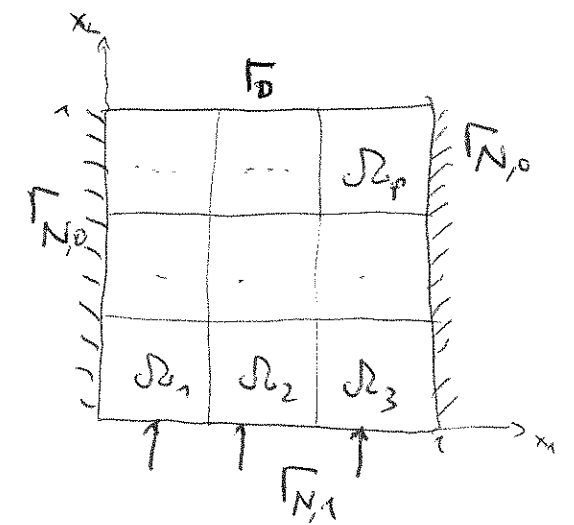
\includegraphics[width = 0.4 \textwidth]{Bilder/ThermischerBlock.png}
  \caption{Skizze des Thermischen Blocks}{(aus dem Online-Skript von Prof. Dr. Haasdonk zu Reduzierte Basen 2015)}
  \label{fig:ThermischerBlock}
\end{figure}

\begin{itemize}
	\item $(0,1)^2=: \Omega$ zerlegt in $B_1 \cdot B_2 =: p$ kongruente Rechtecke
	\item $\p := [\mu_{min}, \mu_{max}]^p \subset \R^p$ Parameterbereich mit $0 < \mu_{min} < \mu_{max}$
	\item $\mu = (\mu_1,\dots,\mu_p)^T \in \p$ Vektor aus Wärmeleitungskoeffizienten der Teilgebiete, $\kappa(x;\mu)$ stückweise konstante Wärmeleitfähigkeit
	\[
		\kappa(x;\mu) := \sum\limits_{q=1}^p \mu_q \cdot \chi_{\Omega_q}(x)
	\]
	\item elliptische PD mit Dirichlet- \& Neumann Randbedingungen:
	\begin{align*}
	- \nabla \cdot (\kappa(x;\mu) \nabla u(x;\mu)) &= 0 &\text{ für } x \in \Omega \\
	u (x;\mu) &= 0 &\text{ für } x \in \Gamma_D \\
	\kappa(x;\mu) \nabla u(x;\mu) \cdot n(x) &= i &\text{ für } x \in \Gamma_{N,i} \,\, , \, \, i=0,1
	\end{align*}
	Anschauung: ``Kühlung'' auf $u=0$ auf $\Gamma_D$, ``Isolierung'' an $\Gamma_{N,0}$ und Einheits-Wärmefluss auf $\Gamma_{N,1}$, keine Wärmequellen.
	
	schwache Form: gesucht $u(\mu) \in H^1_{\Gamma_D}(\Omega) := \{u \in H^1(\Omega) | u_{|\Gamma_D}=0\}$ s.\,d.
	\[
		\int_{\Omega} \kappa(x;\mu) \nabla u(x;\mu) \cdot \nabla v(x) dx = \int_{\Gamma_{N,1}} v(x) dx \qquad \forall \, v \in H^1_{\Gamma_D}(\Omega)
	\]
	\item Ausgabe: Mittlere Temperatur auf $\Gamma_{N,1}$
	\[
		s(\mu) := \int_{\Gamma_{N,1}} u(x;\mu) dx
	\]
	\item Man kann zeigen, dass dies ein Problem von Typ $\prob$ darstellt. Insbesondere ist $a(\pdot,\pdot;\mu)$ separierbar parametrische stetige Bilinearform, gleichmäßig beschränkt, glm. koerziv und Lipschitz-stetig bzgl. $\mu$. Ebenso ist $f(\pdot;\mu)$ eine separierbar parametrische stetige Linearform, gleichmäßig beschränkt und Lipschitz-stetig bzgl. $\mu$. $\rightarrow$ Übung
	\item Modell erlaubt einfache aber interessante Einblicke in Struktur von $\LM$:
	\begin{enumerate}[1.]
		\item einfache Lösungsstruktur: Falls $B_1 =1$ (oder $B_1>1$ aber identische $\mu_i$ pro Zeile) besitzt die Lösung horizontale Symmetrie. Man kann zeigen: $u(\mu)$ ist stückweise linear und enthalten in einem $B_2$-dimensionalen (also insbesondere endlichdimensionalen) Teilraum von $H^1_{\Gamma_D}(\Omega)$. (Übung)
		\item komplexe Lösungsstruktur: Falls $B_1>1$ und $\mu \in \p$ beliebig existieren keine Symmetrien, man findet keinen endlichdimensionalen Raum, der alle $u(\mu)$ enthält
		\item Parameterredundanz: $\LM$ ist invariant bzgl. Skalierung von $\mu$, d.\,h. falls $u(\mu)$ ist Lösung von $\prob$, so ist $u(c\mu) = \frac{1}{c}u(\mu)$ Lösung von $\prob[c\mu]$.
	\end{enumerate}
	\textsf{demo\_detailed\_gui.m}: Beispiele für Parametervariation \& Lösungen. 
\end{itemize}
\end{bsp}

\begin{bsp}[Matrixgleichung] \beginwithlist
	\begin{itemize}
		\item Zu $\mu \in \p$ suche $u(\mu) \in \R^H$ als Lösung von
			\[
				A(\mu) u(\mu) = b(\mu)
			\]
			für $A(\mu) \in \R^{H \times H}$ und $b(\mu) \in \R^H$.
		\item Dies ist Beispiel für $\prob$ via
			\[
				X := \R^H, \quad a(u,v;\mu) := v^\top A(\mu) u, \quad f(v;\mu) := v^\top b(\mu)
			\]
			und beliebiger linearer Ausgabe $l(v;\mu) := \ubar l^\top v$ für $\ubar l \in \R^H$.
	\end{itemize}
\end{bsp}

\begin{bsp}[$Q_a = 1$]
	Falls $a(\pdot,\pdot;\mu)$, $f(\pdot;\mu)$ separierbar parametrisch mit $Q_a = 1$ und $Q_f$ beliebig, so ist $\LM$ enthalten in einem $Q_f$-dimensionalen linearen Teilraum von $X$:
	\[
		\prob \quad \Rightarrow \quad \Theta_a^1(\mu) a^1(u,v) = \sum_q \Theta_f^q(\mu) f^q(v) \quad \forall v \in X
	\]
	$\Theta_a^1(\mu) \neq 0$ wegen $a$ gleichmäßig koerziv
	\[
		a^1(u,v) = \sum_q \frac{\Theta_f^q(\mu)}{\Theta_a^1(\mu)} f^q(v) \quad \forall v \in X \tag{$*$}
	\]
	$a^1(\pdot,\pdot)$ ist koerziv, $f^q$ linear und stetig
	\begin{align*}
		&\stackrel{\text{Lax-Milgram}}{\Rightarrow} \text{ex. } u^q, q=1,\dots,Q_f \text{ mit } a^1(u^q,v) = f^q(v), \quad v \in X\\
		&\Rightarrow u := \sum_q \frac{\Theta_f^q(\mu)}{\Theta_a^1(\mu)} u^q \text{ löst } (*) \text{ wegen Linearität}\\
		&\Rightarrow u \in \op{span}\{u^q\}_{q=1}^{Q_f}
	\end{align*}
\end{bsp}

\begin{bsp}[$\prob$ mit vorgegebener Lösung]
	Sei $u : \p \to X$ beliebig komplizierte Abbildung.
	Dann existiert ein $\prob$ mit $u(\mu)$ als Lösung via Skalarprodukten:
	\[
		a(v,w;\mu) := \dotp{w}{v}_X, \quad f(v;\mu) := \dotp{u(\mu)}{v}_X
	\]
	d.h.\ Klasse der Probleme $\prob$ können beliebig komplizierte, nichtglatte oder sogar unstetige Lösungsmannigfaltigkeit $\LM$ besitzen.
\end{bsp}

\begin{bem}[Parameter-Anzahl und Lösungskomplexität]
	Es gibt (sogar in der Literatur) ein Missverständnis zwischen Parameteranzahl $p \in \N$ und Komplexität der Lösungsmannigfaltigkeit $\LM$, denn es kann Redundanz in Parametern vorliegen (siehe Thermischer Block).
	Extremfall: $p \in \N$ beliebig, für geeignetes $a(\pdot,\pdot;\mu)$, $f(\mu)$ hat $\prob$ ein $\LM$, welches in einem 1D-Raum enthalten ist. (Übung)
	Beispiel 2.13 zeigt andererseits einen anderen Extremfall: Sogar für $p=1$ kann bei geeignetem $\prob$ das $\LM$ beliebig kompliziert sein (z.B. ``Raumfüllende Kurve'').
	Unter geeigneter Annahmen an $a(\pdot,\pdot;\mu)$ und $f(\pdot;\mu)$ können einfache Regularitätseigenschaften von $u(\mu)$ bzw.\ $\LM$ geschlossen werden.
\end{bem}

\begin{kor}[Beschränktheit von $\LM$]
	Weil $a(\pdot,\pdot;\mu)$ gleichmäßig koerziv und $f(\pdot;\mu)$ gleichmäßig beschränkt, so ist $\LM$ beschränkt
	\[
		\LM \subseteq B_{\frac{\bar\gamma_f}{\bar\alpha}}(0)
	\]

	\begin{proof}
		Klar weil $\norm{u(\mu)} \leq \frac{\bar\gamma_f}{\bar\alpha}$ nach Satz 2.8.
	\end{proof}
\end{kor}

\begin{satz}[Lipschitz-Stetigkeit]
	Falls $a(\pdot,\pdot;\mu)$, $f(\pdot;\mu)$, $l(\pdot;\mu)$ Lipschitz-stetig bzgl.\ $\mu$, so sind $u(\mu)$ und $s(\mu)$ Lipschitz-stetig bzgl.\ $\mu$ mit Lipschitz-Konstanten
	\[
		L_u = \frac{L_f}{\bar\alpha} + \bar\gamma_f \frac{L_a}{\bar\alpha^2} \quad \text{und} \quad L_s = L_l \frac{\bar\gamma_f}{\bar\alpha} + \bar\gamma_l L_u
	\]

	\begin{proof}
		Übung.
	\end{proof}
\end{satz}

\begin{satz}[Diffbarkeit]
	Sei $a(u,\pdot;\mu) \in X'$ Frechet-diffbar in Umgebung von $(u_0,\mu_0) \subset X \times \p$ und $f(\pdot; \mu) \in X'$ Frechet-diffbar in Umgebung von $\mu_0 \in \p$.
	Dann ist Lösung $u(\mu)$ von $\prob$ Frechet-diffbar in Umgebung von $\mu_0 \in \p$ mit
	\[
		\D_\mu u(\mu) := -\left(\pd{u} F(u,\mu) \right)^{-1} \pd{\mu} F(u,\mu)
	\]
	wobei $F(u,\mu) := a(u,\pdot;\mu) - f(\pdot;\mu) \in X'$.

	\begin{proof}
		Aus Frechet-Diffbarkeit von $a(\pdot,\pdot;\pdot)$ und $f(\pdot;\pdot)$ folgt Frechet-Diffbarkeit von $F : X \times \p \to X'$ in Umgebung von $(u_0,\mu_0)$ mit partiellen Ableitungen
		\[
			\pd{\mu} F(u_0,\mu_0) := \pd\mu a(u_0,\pdot;\mu_0) - \pd\mu f(\pdot;\mu_0) \in L(\R^p,X')
		\]
		und $\pd u F(u_0,\mu_0) \in L(X,X')$ durch
		\[
			\pd u F(u_0,\mu_0) h_u := a(h_u,\pdot;\mu_0) \in X' \quad \forall h_u \in X
		\]
		Dann erfüllt $u(\mu)$ als Lösung von $\prob$ gerade
		\[
			F(u(\mu),\mu) = 0
		\]
		in Umgebung von $\mu_0$.
		Dann ist (z.B. mit Folgerung 2.15 in Ruzicka: Nichtlineare Funktionalanalysis, Springer 2004) auch $u(\mu)$ Frechet-diffbar in Umgebung von $\mu_0$ mit Ableitung
		\[
			\D_\mu u(\mu) := -\left(\pd u F(u,\mu) \right)^{-1} \pd\mu F(u,\mu)
		\]
	\end{proof}
\end{satz}

\begin{bem} \beginwithlistbem
	\begin{itemize}
		\item Plausibilität der Ableitungsformel folgt aus formellem Ableiten:
			\begin{align*}
				&&\D_\mu \left(F(u(\mu),\mu)\right) &= 0 &\\
				&\Rightarrow& \pd u F(u(\mu),\mu) \D_\mu u(\mu) + \pd\mu F(u,\mu) &= 0 &\\
				&\Rightarrow& \pd u F(u(\mu),\mu) \D_\mu u(\mu) &= -\pd\mu F(u,\mu) &\\
				&\Rightarrow& \D_\mu u(\mu) &= -\left(\pd u F(u(\mu),\mu) \right)^{-1} \pd\mu F(u,\mu) &
			\end{align*}
		\item Man kann zeigen, dass die Sensitivitäts-Ableitungen $\partial_{\mu_i} u(\mu) \in X$ für $i = 1,\dots,p$ erfüllen das sogenannte \emph{Sensitivitätsproblem}
			\[
				a(\partial_{\mu_i} u(\mu),v;\mu) = \tilde f_i(v;u(\mu),\mu)
			\]
			mit rechter Seite $\tilde f_i(\pdot; u(\mu),\mu) \in X'$ gegeben durch
			\[
				\tilde f_i(\pdot;w,\mu) := \partial_{\mu_i} f(\pdot;\mu) - \partial_{\mu_i} a(w,\pdot;\mu)
			\]
			d.h.\ das Problem $\prob$ mit modifizierter rechter Seite, in welcher insbesondere $u(\mu)$ eingeht. (Übung)
		\item Hinreichend für die Diffbarkeit von $a$, $f$ in Satz 2.16 sind z.B.\ im Fall von separierbarer Parameterabhängigkeit die Diffbarkeit der Koeffizienten $\Theta_a^q(\mu)$, $\Theta_f^q(\mu)$, $q = 1,\dots$ (Übung)
		\item Ähnliche Aussagen / Sensitivitätsprobleme gelten für Ableitungen höherer Ordnung.
			Also überträgt sich Glattheit der Koeffizientenfunktionen auf Glattheit der Lösung / Mannigfaltigkeit.
	\end{itemize}
\end{bem}
